% # -*- coding: utf-8 -*-
\section{Evaluation} \label{seciton:evaluation}
\subsection{Security Capability}

% 評価として,提案するセキュリティ機構を適用したカーネルにおいて,特権奪取攻撃か
% ら権限情報保護が適切に動作するかの調査を目的とする.セキュリティ機能評価の項目
% と内容を以下に示す.
The security capability evaluation validates whether the kernel with the
KDPM adequately protects privileged information.
% properly protect privilege information.
% from privilege-grabbing attacks. The items and contents of the security function
% evaluation are listed below.

% %\begin{enumerate}%[leftmargin=1.0cm,topsep=0pt ]\itemsep=-1.0ex \parskip=1.0ex
\begin{enumerate}%[topsep=0pt]%\itemsep=-1.0ex \parskip=1.0ex  

% \item 特権奪取攻撃に対するセキュリティ機能の評価
\item Prevention of privilege escalation attack\\
%   提案するセキュリティ機構を適用したカーネルに対して,特権奪取攻撃に利用可能な
%   カーネル脆弱性を導入し,特権奪取攻撃を行うユーザプロセスを実行する.
%   %
%   予め権限情報Protection keyの書込み制限を有効化,特権奪取攻撃実行時に,権限情
%   報の改ざん防止を実現可能か評価した.
%
% A kernel vulnerability that can be used for a privilege escalation attack is
% introduced into the kernel with the proposed security mechanism applied, and a
% user process that performs a privilege escalation attack is executed.
%
A kernel vulnerability that can be exploited for a privilege escalation attack is
introduced into the Linux kernel.
%
% We evaluate 
The evaluation of the kernel with Implementation 1 enables the write
restriction of the privileged information of user processes. This prevents an
adversary from performing a privilege escalation attack.
% to prevent an adversary's
% user process, which performs a privilege escalation attack. 

\item Preventing the defeat of security mechanism\\
The evaluation of the kernel with Implementation 2 enables the write
restriction of kernel data of the LSM to prevent MAC defeat.%the defeat of MAC. 


% We evaluated the security capability of the kernel with the proposed security mechanism
% preventing the falsification of authorization
% information by enabling the writing restriction of authorization information
% protection keys in advance, and by preventing the falsification of authorization
% information when a privilege-grabbing attack is executed.
\end{enumerate}

\subsection{Performance Evaluation}

% 提案するセキュリティ機構を適用したカーネルのセキュリティ機能評価は先行研究におい
% て示している\cite{kzn21css}.本稿では,

% 性能評価として,実現方式1に対して,ベンチマーク測定によるカーネルとユーザプロ
% セスへの動作影響有無の調査,および実現方式2で用いるPKS操作による性能への影響を
% 確認した.評価項目と内容を以下に示す.

% In performance evaluation, we investigate whether the kernel and user processes
In performance evaluation, investigation results indicate whether the kernel and
user processes are affected by Implementation 1 and the effect of the PKS
operations used in Implementation 2.
% both
% in implementation 2.

% we investigated whether or not the kernel and user
% processes were affected by benchmark measurements for implementation method 1,
% and confirmed the effect of PKS operations used in implementation method 2 on
% performance. The evaluation items and their contents are listed below.

\begin{enumerate}%[topsep=0pt]%\itemsep=-1.0ex \parskip=1.0ex

% \item カーネル処理におけるオーバヘッド\\
\item Measurement of the kernel performance overhead\\
%     %
%     実現方式1を適用した Linux カーネルにおいて,ベンチマークソフトウェアを用いたシ
%     ステムコールのオーバヘッドの測定した.
To measure the performance of the Linux kernel with Implementation 1, the benchmark
software calculates the overhead of the system call invocation latency.

%   \item PKS操作におけるオーバヘッド\\
\item Measurement of PKS performance overhead\\
%     %
%     提案するセキュリティ機構で用いる PKS の利用にかかるオーバヘッドとして,PKS 操
%     作に関する処理時間を測定した.
% To measure the performance of the PKS in the KDPM, we measure the processing
To measure the performance of the PKS in the KDPM, the measurement result
indicates the processing time of the PKS operations in the Linux kernel with
Implementation 2.
%Specifically, we measured the processing time of PKS operations in the Linux kernel.
% We measured the overhead of using PKS in the proposed security mechanism.
% Specifically, we measured the processing time related to PKS operations.

\item Measurement of the kernel instruction increase\\
To measure the instruction insertion of the Linux kernel with implementations,
the disassembling tool indicates the additional instructions. 

\end{enumerate}
  

% \subsection{Tracing and Identification Capability}
% %\reduline{
% The ability of vkTracer to identify vulnerable kernel code information, when an
% adversary's user process attempts to exploit a proven kernel vulnerability in
% invoking a system call, was evaluated.
% %
% The assessment of vkTracer was validated by identifying the vulnerable kernel
% code. 



% \subsection{Performance Measurement}
% To evaluate the performance costs of tracing, identification, kernel, and 
% user process overhead were measured.

% \begin{enumerate}%[leftmargin=0.5cm]%\itemsep=-1.0ex \parskip=1.0ex
% \item {\bf Measurement of vulnerable kernel code identification}:
%   %
% %  \reduline{
%     Tracing and identification cost was measured using the PoC
%     applications.
    
% \item {\bf Measurement of the kernel overhead}:
%   To measure the feasibility of tracing for the kernel, LMbench was %and sysbench were
%   used to calculate the overhead of the system call invocation latency.
%   %and system latency.

% \item {\bf Measurement of the application overhead}:
%   The application overhead for the web server and client was measured using nginx and ApacheBench.
    
% \end{enumerate}


\subsection{Evaluation Environment}

\subsubsection{Equipment}
% PKSに対応したCPUは2022年1月時点では提供されていない.評価には CPU Intel(R)
% Core(TM) i7-7700HQ(2.80GHz,4コア),Memory 16 GBytes を備えた計算機を用い,性
% 能評価を行う仮想計算機環境として PKS に対応したQEMU 6.0.91を用いた \cite{qemu}.
% %
% QEMU上のゲストOSは Debian 10.2 とし,実現方式1を Linux kernel 5.3.18 を対象
% に,15個のファイルに対して431行を追加し実装した.また,PKS操作の性能負荷評価のた
% めの専用の測定プログラムとして165行を Linux カーネル に追加した.


%  containing one environment server and a log collection
% server.
%
%The environment for the evaluation of the performance cost was
% The environment for the PoC code, kernel, and web server for measuring
% The environment for the PoC code, kernel for 
% measuring the performance cost was implemented 
% The evaluation environment for 
% We evaluated the PoC code and kernel using a physical machine equipped with an
The evaluation environment for PoC code and kernel was a physical machine
equipped with an Intel (R) Core (TM) i7-7700HQ (2.80 GHz, x86\_64) processor
with 16 GB memory.
%
% The web client machine was equipped with an Intel (R) Core (TM)
% i5-4200U (1.6 GHz) processor with 8 GB of memory, running on Windows 10.
%

The security capability evaluation was implemented on a virtual machine because
QEMU 6.0.91 supports the PKS. However, the PKS is not available as of January
2022 on the Intel CPU.
%
The guest OS on QEMU was Debian 10.2, and implementations required 15 source
files and 431 lines for Linux kernel 5.3.18.
%
% In addition, 
% The performance evaluation of the PKS operation require the measurement program
The PKS performance for Implementation 2 was evaluated using a
measurement program that required 165 lines for Linux kernel 5.3.18.
% for the purpose of measuring the performance of the system
% was added to the Linux kernel, 

%% \reduline{
% The network environment for the application benchmark was a 1
% Gbps hub supporting direct connections between the server and client
% machines.

% \subsubsection{特権奪取攻撃に利用可能なカーネル脆弱性}

\subsubsection{Implementation}
%
%\reduline{
% vkTracer was implemented on the Linux x86\_64 CPU kernel.
%
To evaluate the security capability, a kernel vulnerability was introduced into
% the Linux kernel using a PoC code \cite{CVE-2017-6074} that leads to privilege
the Linux kernel using a PoC code \cite{CVE-2017-16995} that leads to privilege
escalation via memory corruption through the system call number 350.
%
% One kernel vulnerability 
Additionally, the Linux kernel module (LKM) attempted to overwrite the LSM function pointer to
defeat the MAC on the running kernel:
% which can be used for privilege escalation attacks 

\begin{itemize}%[topsep=0pt]
  
  %\item {\bf Memory Corruption}: The vulnerable kernel code 1 is
\item {\bf Privilege escalation:} Vulnerable kernel code 1 refers to
  CVE-2017-16995 \cite{CVE-2017-16995}, which was implemented as a system call
  \verb|sys_kvuln01|.
  %, \verb|support_sys_kvuln01_01|, and \verb|support_sys_kvuln01_02|.
  %
  The PoC code exploits the vulnerable kernel code to overwrite the privileged
  information of a user process for privilege escalation.

  \item {\bf Defeating security mechanism:} A customized LKM attempts to overwrite
  the function pointer of the kernel code that manages the LSM file access
  permission to circumvent the MAC decision.

\end{itemize}

% 提案するセキュリティ機構のセキュリティ機能評価のため,特権奪取攻撃に利
% 用可能な独自システムコールをシステムコール番号350としてカーネルに導入
% した.

% \vspace{-2.0ex}
% \begin{itemize}\topsep=-1.0ex \itemsep=-1.0ex \parskip=1.0ex  
  
% \item カーネル脆弱性(特権奪取):独自システムコールを実行中,権限
%   情報を変更するカーネル関数を呼出し,ユーザプロセスの権限情報を管理者
%   ユーザに変更する.

% \end{itemize}
% \vspace{-2.0ex}

% 評価において,独自システムコールを呼出すPoCコードをユーザプロセス経由
% にて実行し,特権奪取攻撃を行い,一般ユーザから管理者ユーザへの変更を
% 試みる.

% \subsubsection{特権奪取攻撃を行う独自システムコールの捕捉}
\subsection{Security Capability Evaluation Result}
\subsubsection{Prevention of Privilege Escalation Attack}
% 攻撃を行うユーザプロセスによる独自のシステムコール捕捉時の動作結果を
% \figref{fig:kvuln1_1_04}に示す.
% of the operation when an original system call
The security evaluation result for the adversary's user process is shown in
Figure \ref{fig:kvuln1_1_04}.
% %
% \figref{fig:kvuln1_1_04} の3行目にて,プロセスID 1661の独自システムコール(シ
% ステムコール番号 350)の呼出しを捕捉している.5行目,および6行目にて,PKRS は
% 0x8 であり,Protection key 1 の書込み制限(WD1)は有効化されている.
In line 3, the kernel captures the original system call (i.e., system call
number 350) with process ID 1661. The kernel indicates 0x8, which indicates that
the write disable (WD) of Pkey 1 is enabled.
% %
% 10行目において,Protection key 1 の権限情報を格納するページへの書込みが行われ
% た際,ページフォルト(エラー番号 35)を捕捉している.捕捉されたページフォルト
% は Protection key により保護されたページへの書込み保護違反を示している.
In line 10, the kernel catches a page fault (i.e., error number 35) when writing
to the page that stores the privileged information with Pkey 1. The page fault
indicates a write protection violation of a page protected by the Pkey. In line
14, the kernel sends \verb|SIGKILL| to the user process of the adversary.

%
% 評価においては,特権奪取攻撃の動作確認のため,14行目から15行目にかけて,
% ページフォルト捕捉後,PKRS に 0x0 を書込み,Protection key 1 への書込
% み制限(WD1)を無効化し,特権奪取が成功することを確認している.
% In the evaluation, %we confirmed the operation of the privilege escalation attack,

% From the evaluation result, we confirmed that Linux kernel with the proposed
% security mechanism prevents privilege escalation attacks. The proposed mechanism
% can correctly handle the management of the Pkey and detect the memory
% corruption of a vulnerable kernel code.
% 1 after the page fault is caught, from line 14 to 15.

% writing 0x0 to PKRS and disabling the write restriction (WD1) to Protection key
% 1 after the page fault is caught, from line 14 to 15.

% \subsubsection{Prevention of Defeating Security Mechanism:}
\subsubsection{Preventing the Defeat of Security Mechanism}
% 攻撃を行うユーザプロセスによる独自のシステムコール捕捉時の動作結果を
% \figref{fig:kvuln1_1_04}に示す.
% of the operation when an original system call
The security evaluation result of the LKM is shown in Figure
\ref{fig:defeat_mac}.
% %
% \figref{fig:kvuln1_1_04} の3行目にて,プロセスID 1661の独自システムコール(シ
% ステムコール番号 350)の呼出しを捕捉している.5行目,および6行目にて,PKRS は
% 0x8 であり,Protection key 1 の書込み制限(WD1)は有効化されている.
In line 2, the LKM attempts to find one of the function pointers of
\verb|selinux_hooks|. In line 5, LKM attempts to overwrite the function pointer of
\verb|selinux_hooks|.
% the kernel captured the original system call (i.e., system call
% number 350) with process ID 1661. The kernel indicates 0x8, which indicates that
% the write disable (WD) of Pkey 1 is enabled.
% %
% 10行目において,Protection key 1 の権限情報を格納するページへの書込みが行われ
% た際,ページフォルト(エラー番号 35)を捕捉している.捕捉されたページフォルト
% は Protection key により保護されたページへの書込み保護違反を示している.
In line 7, the kernel catches a page fault (i.e., error number 35) when writing
to the page storing the function pointer with Pkey 1. The page fault
indicates a write protection violation of a page protected by Pkey.
% In line 14, the kernel sends \verb|SIGKILL| to the user process of the adversary.

%
% 評価においては,特権奪取攻撃の動作確認のため,14行目から15行目にかけて,
% ページフォルト捕捉後,PKRS に 0x0 を書込み,Protection key 1 への書込
% み制限(WD1)を無効化し,特権奪取が成功することを確認している.
% In the evaluation, %we confirmed the operation of the privilege escalation attack,

%From the security evaluation results, we confirmed that the Linux kernel with the
From the security evaluation results, the Linux kernel with the KDPM prevents
privilege escalation attacks and avoids the defeat of security mechanism were
confirmed. The KDPM correctly manages the Pkey and detect memory corruption of
the vulnerable kernel code.

% \begin{figure}[t]
%   \begin{center}
%   \hspace*{-8.5ex}    
%     \begin{tabular}{cc}

%       \begin{minipage}[t]{0.67\hsize}
%         % \begin{figure}[tb]
%         \begin{center}
%         % \hspace*{-09.0ex}
%           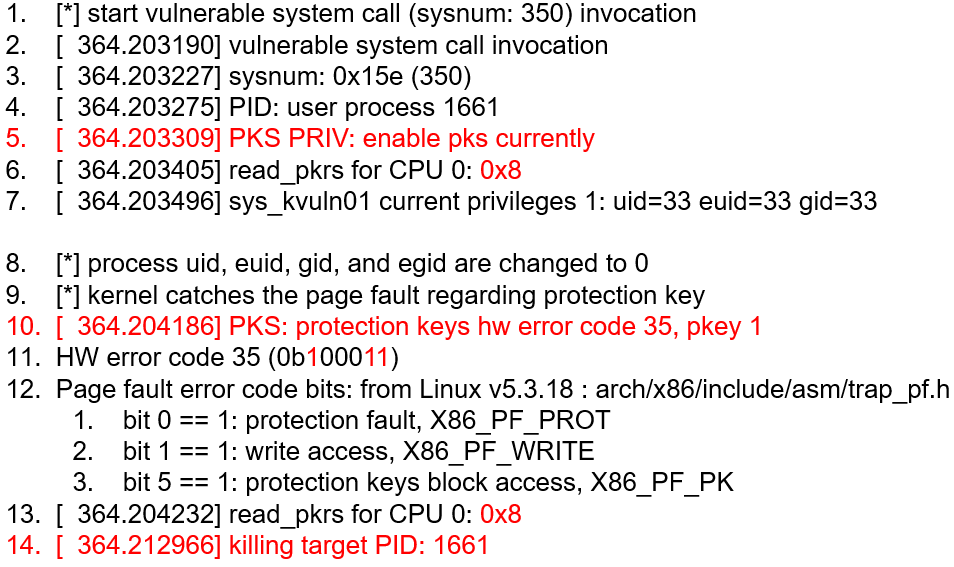
\includegraphics[bb=0 0 716 425, scale=.325]{./imgs/008_screenshot_2021-08-18_3.35.12.png}
%         \end{center}
%         % \vspace{-2.0ex}
%         \caption{
%         %
%         % 特権奪取攻撃に利用可能なシステムコール捕捉時の動作結果
%         Attack prevention of privilege escalation
%         %実現方式を適用した権限情報カーネルデータの保護
%         %
%         }
%         % \vspace{-4.5ex}
%         \label{fig:kvuln1_1_04}
%         %\end{figure}
%       \end{minipage} &

%       \begin{minipage}[t]{0.67\hsize}
%         \begin{center}
%         %\hspace*{-09.0ex}
%           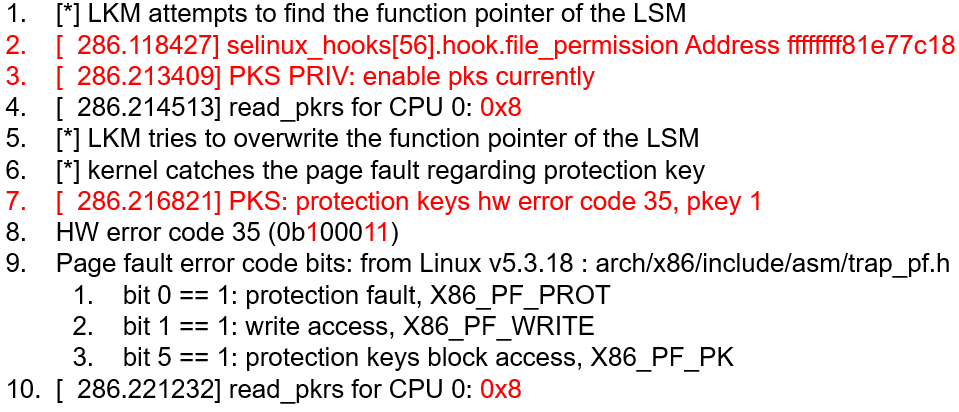
\includegraphics[bb=0 0 719 309, scale=.325]{./imgs/009_screenshot_2021-08-18_3.35.12.png}
%         \end{center}
%         % \vspace{-2.0ex}
%         \caption{
%         %
%         % 特権奪取攻撃に利用可能なシステムコール捕捉時の動作結果
%         Attack prevention of defeating MAC
%         %実現方式を適用した権限情報カーネルデータの保護
%         %
%         }
%         % \vspace{-4.5ex}
%         \label{fig:defeat_mac}
%         %\end{figure}
%       \end{minipage}
%     \end{tabular}
%   \end{center}
% \end{figure}

\begin{figure}[t]
  \begin{center}
    % \hspace*{-09.0ex}
      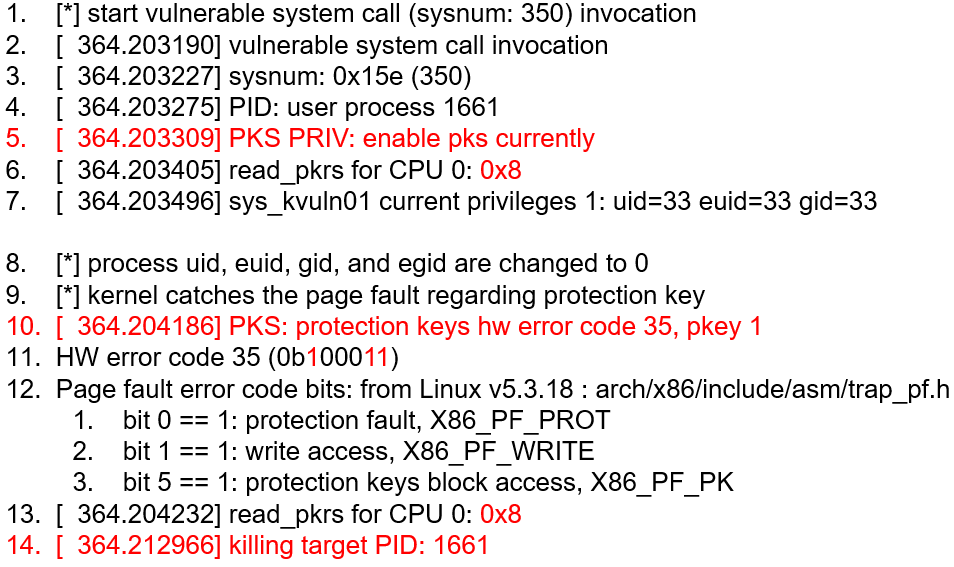
\includegraphics[bb=0 0 716 425, scale=.325]{./imgs/008_screenshot_2021-08-18_3.35.12.png}
    \end{center}
    % \vspace{-4.0ex}
    \caption{
    %
    % 特権奪取攻撃に利用可能なシステムコール捕捉時の動作結果
    Prevention of a privilege escalation attack
    %実現方式を適用した権限情報カーネルデータの保護
    %
    }
    % \vspace{-2.0ex}
    \label{fig:kvuln1_1_04}
\end{figure}

\begin{figure}[t]
  \begin{center}
    %\hspace*{-09.0ex}
      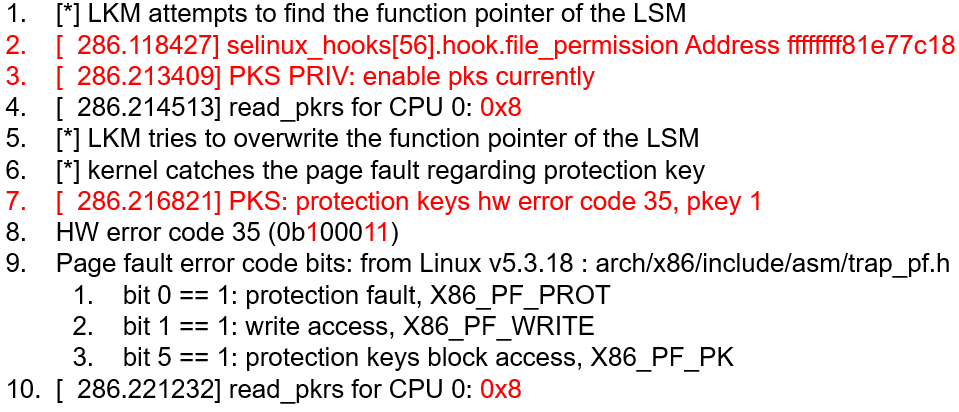
\includegraphics[bb=0 0 719 309, scale=.325]{./imgs/009_screenshot_2021-08-18_3.35.12.png}
    \end{center}
    % \vspace{-4.0ex}
    \caption{
    %
    % 特権奪取攻撃に利用可能なシステムコール捕捉時の動作結果
    Prevention of a MAC defeat
    %実現方式を適用した権限情報カーネルデータの保護
    %
    }
    % \vspace{-2.0ex}
    \label{fig:defeat_mac}
\end{figure}

% \begin{figure}[tb]
%   \begin{center}
% %    \hspace*{-09.0ex}
%     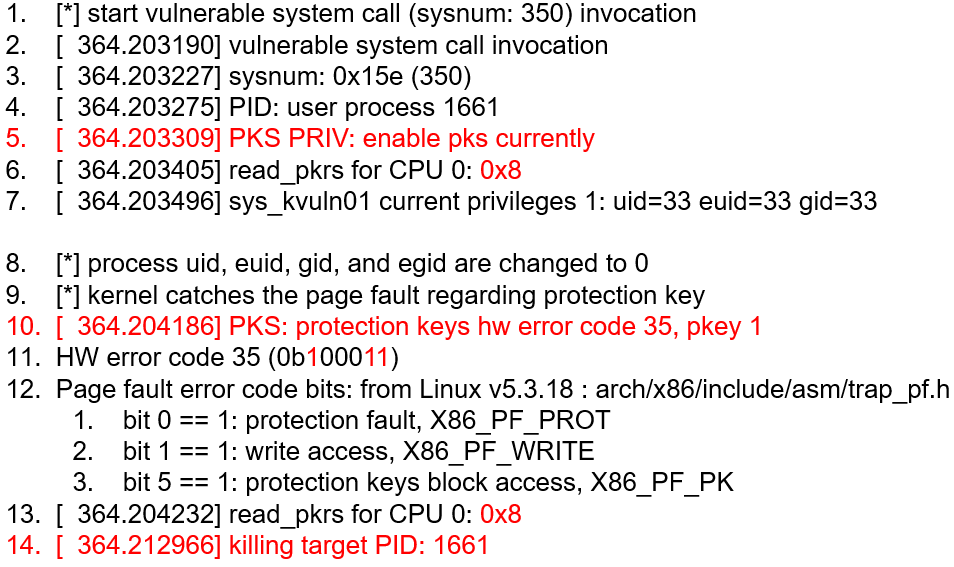
\includegraphics[bb=0 0 950 589, scale=.260]{./imgs/008_screenshot_2021-08-18_3.35.12.png}
%   \end{center}
%   \vspace{-2.0ex}
%   \caption{
%     %
%     特権奪取攻撃に利用可能なシステムコール捕捉時の動作結果
%     %
%   }
%   \vspace{-4.5ex}
%  \label{fig:kvuln1_1_04}
% \end{figure}


% \subsection{カーネル処理におけるオーバヘッド}
\subsection{Performance Evaluation Result}

\subsubsection{Measurement of the Kernel Processing Overhead}

% 実現方式1のカーネル負荷として,システムコールのオーバヘッドの測定をベンチマーク
% ソフトウェア LMbench により評価した.LMbenchを実現方式1の適用前のLinux kernel と
% 適用したLinux kernelにてそれぞれ10回実行し,平均値からシステムコールのオーバヘッ
% ドを算出した.
The system call overhead was measured using LMbench benchmark software. 
%
A vanilla kernel was compared with the kernel with Implementation 1.
LMbench was executed 10 times to calculate the average system call latency.
% as the kernel load of the implementation method 1. 10 times LMbench was run on the
% Linux kernel before and after the application of the implementation method 1,
% respectively, and the average value was calculated as the system call overhead.

% 評価結果を表\ref{tb:evaluation_qemu_lmbench1}に示す.LMbench では, fork+/bin/sh
% は54回,fork+execveは4回,fork+exitは2回,open/close は2回,および,その他は1回
% のシステムコール呼出しを行う.
LMbench performs 54 invocations of the system call for fork+/bin/sh, 4 invocations
for fork+execve, 2 invocations for fork+exit and open/close, and 1
invocation each of the other system calls.
% %
% 表\ref{tb:evaluation_qemu_lmbench1}から,提案するセキュリティ機構の適用時におい
% て,最もオーバヘッドの発生したシステムコール処理はfork+execveであり,9.01\% %X.XXX $\mu$s
% を示した,また,最も少ないオーバヘッドはstatであり,2.96\%を示した.
% %
Table \ref{tb:evaluation_qemu_lmbench1} shows the overhead of the system call. The
highest and lowest overheads are fork+execve with 9.01\% and stat with 2.96\%,
respectively.

% -*- coding: utf-8; mode: latex; -*-
\begin{table}[t]
    \centering
    %  \caption{Overhead of MKM mechanism on the Linux kernel ($\mu$s)}
    \caption{System call invocation overhead of Implementation 1 ($\mu$s)}
  %  \vspace{-2.5ex}
    \scalebox{0.85}{
  
      \begin{tabular}{lrrr}
        \hline \noalign{\smallskip}
        \begin{tabular}{l}
          {\bf System call}
        \end{tabular}
        &
        \begin{tabular}{l}
          {\bf Vanilla kernel}
        \end{tabular}
        &
        \begin{tabular}{l}
          {\bf Implementation 1}
        \end{tabular}
        &
        \begin{tabular}{l}
          {\bf Overhead}
        \end{tabular}
        \\
        \noalign{\smallskip}
        \hline
        \noalign{\smallskip}
  fork+/bin/sh & 227111.28  & 236738.69  & 9627.41 (4.24\%)  \\
  fork+execve  & 12780.0566 & 13931.6703 & 1151.6136 (9.01\%)    \\
  fork+exit    & 10837.0729 & 11285.5603 & 448.4874 (4.14\%)    \\
  open/close   & 1302.5639  & 1334.5312  & 41.9672 (2.95\%)     \\
  read         & 168.8898   & 180.4594   & 11.5696 (6.85\%) \\
  write        & 164.2567   & 176.4273   & 12.1705 (7.41\%)     \\
  fstat        & 195.0063   & 203.7508   & 8.7445  (4.48\%)     \\
  stat         & 613.7426   & 631.9393   & 18.1966 (2.96\%)     \\
        
  \noalign{\smallskip}
  \hline
  \noalign{\smallskip}
      \end{tabular}
    }    
      \label{tb:evaluation_qemu_lmbench1}
  %  \vspace{-2.0ex}
  \end{table}
   % lmbench

% \subsection{PKS操作におけるオーバヘッド}
\subsubsection{Measurement of PKS Operations}

% PKSの利用にかかる性能評価として,PKS操作に関するオーバヘッドを測定した.専用の測
% 定プログラムにおいて,カーネルにおけるPTEへのPkeyの設定ならびに PKRS 読書きを
% 10,000回繰返す処理を10回行い,平均値を測定した.
% %
% To evaluate the performance of using PKS, we measured the overhead associated
% with PKS operations.
% Measurement of the PKS operations. 
The Linux kernel with Implementation 2 invokes the Pkey write of the PTE and
read and write of the PKRS. The measurement program was repeated 10,000 times, and
the average value was calculated.
% 評価結果について表\ref{tb:evaluation_qemu_cpubench2}に示す.
% %
% Pkey の書込みには 30.5 ns ならびに PKRS の読込みに22.1 ns,書込みに
% 1347.9 nsのオーバヘッドを必要とすることを示した.
Table \ref{tb:evaluation_qemu_cpubench2} shows the cost of the PKS operations.
The write of Pkey required 30.5 ns; PKRS read required 22.1 ns, and PKRS
write required 1347.9 ns.
% was required.

%\begin{table}[t]
\hspace{-22.0ex}
\begin{tabular}{rl}    
  %\centering
   \begin{minipage}{0.8\hsize}    
    %  \caption{Overhead of MKM mechanism on the Linux kernel ($\mu$s)}
    \centering
    \caption{System call invocation overhead of Implementation 1 ($\mu$s)}
  %  \vspace{-2.5ex}
    \scalebox{1.0}{
  
      \begin{tabular}{lrrr}
        \hline \noalign{\smallskip}
        \begin{tabular}{l}
          {\bf System call}
        \end{tabular}
        &
        \begin{tabular}{l}
          {\bf Vanilla kernel}
        \end{tabular}
        &
        \begin{tabular}{l}
          {\bf Implementation 1}
        \end{tabular}
        &
        \begin{tabular}{l}
          {\bf Overhead}
        \end{tabular}
        \\
        \noalign{\smallskip}
        \hline
        \noalign{\smallskip}
  fork+/bin/sh & 227111.28  & 236738.69  & 9627.41 (4.24\%)  \\
  fork+execve  & 12780.0566 & 13931.6703 & 1151.6136 (9.01\%)    \\
  fork+exit    & 10837.0729 & 11285.5603 & 448.4874 (4.14\%)    \\
  open/close   & 1302.5639  & 1334.5312  & 41.9672 (2.95\%)     \\
  read         & 168.8898   & 180.4594   & 11.5696 (6.85\%) \\
  write        & 164.2567   & 176.4273   & 12.1705 (7.41\%)     \\
  fstat        & 195.0063   & 203.7508   & 8.7445  (4.48\%)     \\
  stat         & 613.7426   & 631.9393   & 18.1966 (2.96\%)     \\
        
  \noalign{\smallskip}
  \hline
  \noalign{\smallskip}
      \end{tabular}
    }    
      \label{tb:evaluation_qemu_lmbench1}

   \end{minipage}
   \hspace{8mm}
   \begin{minipage}{0.7\hsize}
    \centering
    \caption{PKS operations overhead of Implementation 2 (ns)}
  %  \vspace{-2.5ex}
    \scalebox{1.0}{
  
      \begin{tabular}{lr}
        % \hline
        \hline \noalign{\smallskip}
        % \hline
        \begin{tabular}{l}
          {\bf Instruction}
        \end{tabular}
        &
        \begin{tabular}{l}
          % {\bf Our proposed mechanism}
          {\bf Implementation 2}
         \end{tabular}
          \\
          \noalign{\smallskip}          
          \hline
          \noalign{\smallskip}
          %Total        & 349.260 \\
          % Pkey read    & 0.xxx  \\
          % Pkey write   & 30.5263  \\
          % PKRS read    & 22.1052  \\
          % PKRS write   & 1347.8965  \\
          Pkey write   & 30.5  \\
          PKRS read    & 22.1  \\
          PKRS write   & 1347.9  \\
          
        \noalign{\smallskip}          
        \hline
        \noalign{\smallskip}          
      \end{tabular}
    }    
      \label{tb:evaluation_qemu_cpubench2}
  \end{minipage}
\end{tabular}
\end{table}
% -*- coding: utf-8; mode: latex; -*-
\begin{table}[t]
    \centering
    %  \caption{Overhead of MKM mechanism on the Linux kernel ($\mu$s)}
    \caption{Overhead of PKS operations (ns)}
  %  \vspace{-2.5ex}
    \scalebox{1.0}{
  
      \begin{tabular}{lr}
        % \hline
        \hline \noalign{\smallskip}
        % \hline
        \begin{tabular}{l}
          {\bf Instruction}
        \end{tabular}
        &
        \begin{tabular}{l}
          % {\bf Our proposed mechanism}
          {\bf Implementation 2}
         \end{tabular}
          \\
          \noalign{\smallskip}          
          \hline
          \noalign{\smallskip}
          %Total        & 349.260 \\
          % Pkey read    & 0.xxx  \\
          % Pkey write   & 30.5263  \\
          % PKRS read    & 22.1052  \\
          % PKRS write   & 1347.8965  \\
          Pkey write   & 30.5  \\
          PKRS read    & 22.1  \\
          PKRS write   & 1347.9  \\
          
        \noalign{\smallskip}          
        \hline
        \noalign{\smallskip}          
      \end{tabular}
    }    
      \label{tb:evaluation_qemu_cpubench2}
  %  \vspace{-2.0ex}
  \end{table} % cpu cycle

\subsubsection{Measurement of the Kernel Instruction Increase}
The Linux kernel with implementations requires protected kernel data management
and handling of write restrictions that contain the instructions of PKS
operations.
%
% The original LKM only contains Pkey write, read, PKRS read and write for the
% measurement of the instructions of PKS operations.
% that contains Pkey and PKRS read, write.
%
For the calculation of the instruction increase, both implementations extract
the additional kernel code to the source code file, then the vanilla kernel only
contains the invocation placement (e.g., function call) of both implementations.
% using same Linux kernel config file.
The disassemble tool calculates instructions for the object files of each
implementation.

% %
Table \ref{tb:evaluation_instructions} shows the increase in instructions.
Implementation 1 requires 176 instructions and Implementation 2 requires 137
instructions.
%  Additionally, PKS operations requires xxx instructions
%
% Additionally, 
%  for both implementations.
% the PKS operations.
% The write of Pkey required 30.5 ns; PKRS read required 22.1 ns, and PKRS
% write required 1347.9 ns.
% -*- coding: utf-8; mode: latex; -*-
\begin{table}[t]
    \centering
    %  \caption{Overhead of MKM mechanism on the Linux kernel ($\mu$s)}
    \caption{Increasing of instructions on the Linux kernel}
  %  \vspace{-2.5ex}
    \scalebox{1.0}{
  
      \begin{tabular}{lrr}
        % \hline
        \hline \noalign{\smallskip}
        % \hline
        % \begin{tabular}{l}
        %   {\bf Instruction}
        % \end{tabular}
        &
        \begin{tabular}{l}
          % {\bf Our proposed mechanism}
          {\bf Implementation 1}
         \end{tabular}
         &
         \begin{tabular}{l}
            % {\bf Our proposed mechanism}
            {\bf Implementation 2}
           \end{tabular}         
        %    &
        %    \begin{tabular}{l}
        %     % {\bf Our proposed mechanism}
        %     {\bf PKS operation}
        %    \end{tabular}                    
          \\
          \noalign{\smallskip}          
          \hline
          \noalign{\smallskip}
          %Total        & 349.260 \\
          % Pkey read    & 0.xxx  \\
          % Pkey write   & 30.5263  \\
          % PKRS read    & 22.1052  \\
          % PKRS write   & 1347.8965  \\
          % Instructions   & xxx.xxx & xxx.xxx \\
          Instructions   & 176 & 137 \\
        %   PKRS read    & 22.1  \\
        %   PKRS write   & 1347.9  \\
          
        \noalign{\smallskip}          
        \hline
        \noalign{\smallskip}          
      \end{tabular}
    }    
      \label{tb:evaluation_instructions}
  %  \vspace{-2.0ex}
  \end{table} % lmbench


% \subsubsection{Implementation}
% %
% %\reduline{
% vkTracer was implemented on the Linux x86\_64 CPU kernel.
% %
% To evaluate the tracing capability, two known kernel vulnerabilities
% were introduced into Linux kernel 5.0.0 using an actual kernel
% vulnerability and PoC code \cite{CVE-2017-6074, CVE-2017-16995}.
% %
% One kernel vulnerability leads to privilege escalation via memory corruption,
% and the other leads to DoS on the running kernel:

% \begin{itemize}
  
%   %\item {\bf Memory Corruption}: The vulnerable kernel code 1 is
% \item {\bf Privilege escalation}: Vulnerable kernel code 1 refers to
%   CVE-2017-6074 \cite{CVE-2017-6074}, which was implemented as system
%   call \verb|sys_kvuln01|, \verb|support_sys_kvuln01_01|, and
%   \verb|support_sys_kvuln01_02|.
%   %
%   PoC code 01 exploits these functions to overwrite the credential
%   information of a user process to achieve privilege escalation.
%   %% カーネル脆弱性1(バッファオーバーフロー):独自システムコール1の
%   %% 実行中,カーネル脆弱性1を含むカーネルコード1-1,1-2を呼出す.ユーザ
%   %% プロセスの権限情報をバッファオーバーフローにより改竄し,特権奪取可能
%   %% とする.

% \item {\bf DoS}:
%   %\item カーネル脆弱性2(解放済みメモリの参照):
%   Vulnerable kernel code 2 refers to CVE-2017-16995 \cite{CVE-2017-16995}, which was
%   implemented as system call \verb|sys_kvuln02| and
%   \verb|support_sys_kvuln02_01|.
%   %
%   PoC code 02 exploits these functions to forcibly free a variable and then free it
%   again (e.g., double free of UAF). The \verb|sys_kvuln02| forces a DoS
%   on the running kernel.
  
%   %% 独自システムコール2の実
%   %% 行中にメモリ領域を確保,カーネルコード2-1を呼出し,該当メモリ領域を
%   %% 開放する.その後,独自システムコール2にて,開放済みメモリ領域を参照
%   %% し,DoS を発生させる.


% \end{itemize}

% %
% In addition, to evaluate the performance cost, vkTracer calculated the
% execution times of the PoC codes. vkTracer required 712 lines for the
% application. The proven kernel vulnerabilities required 192 lines for four
% files, whereas the PoC code for the Linux kernel 5.0.0 had 143 lines.

% \subsection{Identification of Vulnerable Kernel Code} 
% \subsubsection{Case of Privilege Escalation}
% %The left side of Figure \ref{fig:kvuln1_1}
% Figure \ref{fig:kvuln1_1}
% %
% shows that the adversary's user process attempted to invoke the
% %
% \verb|support_kvuln01_01| and \verb|support_kvuln01_02| functions
% during the \verb|sys_kvuln1| system call in lines 6 to 8.
% %
% vkTracer was able to trace and identify the invocation of
% vulnerable kernel codes.% at this time.
% %
% The adversary's user process upgraded from a normal user account (e.g., user id
% is 1000) to obtain the administrator account privilege, as shown by the user
% process id (e.g., user id is 0) at line 10. 
% % changing from the normal user account (e.g., user id is 1000) at line 10.
% %
% Then, vkTracer determined the function names and virtual address ranges
% of the vulnerable kernel codes in lines 18 to 20. This tracing
% result was correct, shown by the symbol information in line 28 to 30.
% %
% Finally, vkTracer generated the profile of \verb|sys_kvlun1| and other functions
% in line 31 to 33.



% \subsubsection{Case of DoS}
% %The right side of Figure \ref{fig:kvuln1_2}
% Figure \ref{fig:kvuln1_2}
% %
% shows that the adversary's user process attempted to invoke the
% %
% \verb|support_kvuln02| and \verb|support_kvuln02_01| functions in lines
% 4 to 7,
% %
% after which the running kernel was terminated. Subsequently, in lines 9 to 10,
% vkTracer determined the function names and virtual address ranges of the
% vulnerable kernel codes at the remote server. This tracing
% result was correct, shown by the symbol information in lines 14 to 15.
% %
% Finally, vkTracer generated the profile of \verb|sys_kvlun2| and
% \verb|support_kvuln02_01| in lines 16 and 17.

% Therefore, vkTracer identified the vulnerable kernel codes and
% extracted the kernel code information as a profile containing the
% function name and virtual address range.


% \subsection{Measurement of The Performance Cost}

% \subsubsection{Measurement of Vulnerable Kernel Code Identification}
% To evaluate the tracing overhead, the processing costs of a vanilla kernel
% and vkTracer were compared.
% %
% The tracing overhead is a measure of the processing time of PoC codes
% that exploit proven kernel vulnerabilities.
% %
% The kernel compilations were run five times to determine the average
% processing time of two different PoC codes as the user process.
% %
% Table \ref{tb:evaluation_physical_kernel} lists the performance scores.
% vkTracer required 5.2728 s and 5.2683 s for the two PoC codes.%, respectively.


% \subsubsection{Measurement of The Kernel Overhead}
% To measure the kernel performance overhead, LMbench was executed five
% times to determine the average system call overhead between a vanilla
% kernel and a kernel with vkTracer.

% LMbench invokes two system call counts for open/close and the other
% system calls count is one.
% %
% Table \ref{tb:evaluation_physical_lmbench} shows that the open/close
% system calls are the highest overhead for vkTracer, i.e., 7.4394 $\mu$s
% (3.7197 $\mu$s for each once), whereas the fstat system call has the
% lowest overhead, i.e., 3.2292 $\mu$s.


% \subsubsection{Measurement of Application Overhead}
% To measure the tracing overhead for the web application,
% %
% the web server nginx 1.21.4 was used, and the benchmark web client was
% ApacheBench 2.4.
% %The web server used was nginx 1.21.4.  The benchmark web client was
% %ApacheBench 2.4.
% The network environment was 1 Gbps.
% %
% % The benchmark configuration adopted the relevant the ApacheBench sending 100,000
% The adopted benchmark configuration involved ApacheBench sending 100,000 HTTP
% accesses and then downloading files for one connection, with file sizes of 1 kB,
% 10 kB, and 100 kB.
% %

% Table \ref{tb:evaluation_physical_apachebench} shows the
% calculation result of the HTTP download request average.
% %
% vkTracer has an average overhead between 0.37 \% and 0.56 \% for each file
% download access.

% %The web application process used was an  web server.
% %The benchmark adopted 
% %for HTTP accesses. 
% %and KPRM implementation 2 has an average overhead of 1.188 \% to 3.008 \% 

%     %\vspace{-4.0ex}
%     %\end{table}
% \begin{table}[t]
%   \centering
%       %\begin{table}[tb]
% %  \vspace{-1.0ex}
%   \caption{Tracing overhead of vkTracer (s)}
% %  \vspace{-1.2ex}          
%         %  \vspace{-2.0ex}
%   \label{tb:evaluation_physical_kernel}
%   \scalebox{0.98}{
%     %  \begin{tabular}{r|r|r|r}
%     \begin{tabular}{lrrr}
%       \hline
% \noalign{\smallskip}      
%       %\begin{tabular}{l}
%       %\end{tabular}
%       %&
%       \begin{tabular}{l}
%         {\bf Application}
%       \end{tabular}
%       &
%       \begin{tabular}{l}
%         {\bf Vanilla kernel}
%       \end{tabular}
%       &
%       \begin{tabular}{l}
%         {\bf w/ vkTracer}
%       \end{tabular}
%       &
%       \begin{tabular}{l}
%         {\bf Overhead}
%       \end{tabular}
%       \\
% \noalign{\smallskip}      
% \hline
% \noalign{\smallskip}
%       PoC code 01  & 0.2047 & 5.4775 & 5.2728 \\            
%       PoC code 02  & 0.1034 & 5.3717 & 5.2683 \\
%       \hline
%     \end{tabular}
%   }
%   %\vspace{-4.0ex}
%   %\end{table}
%   %\vspace{-4.0ex}
% \end{table}

% \begin{table}[t]
%   \centering
%   %\vspace{-1.0ex}
%   \caption{One time system call invocation overhead of vkTracer ($\mu$s)}
%   %\vspace{-1.1ex}  
% %  \vspace{-2.5ex}
%   \scalebox{0.95}{

%     %\begin{tabular}{l|r|r|r}
%     \begin{tabular}{lrrr}
% %      \hline
%       \hline
% \noalign{\smallskip}      
%       \begin{tabular}{l}
%         {\bf System call}
%       \end{tabular}
%       %% &
%       &
%       \begin{tabular}{l}
%         {\bf Vanilla kernel}
%       \end{tabular}
%       &
%       \begin{tabular}{l}
%         {\bf w/ vkTracer}
%       \end{tabular}
%       &
%       \begin{tabular}{r}
%         {\bf Overhead}
%       \end{tabular}        
%         \\
% \noalign{\smallskip}
% \hline
% \noalign{\smallskip}

% open/close & 1.6049 & 9.0443  & 7.4394\\ 
% read	     & 0.3545 & 4.0560  & 3.7015\\
% write	     & 0.2997 & 3.5443  & 3.2446\\
% stat	     & 0.5831 & 3.9714  & 3.3883\\
% fstat	     & 0.4068 & 3.6360  & 3.2292\\

      
%       \hline
%     \end{tabular}
%     \label{tb:evaluation_physical_lmbench}
%   }
%   %\vspace{-2.5ex}
% \end{table}

% \begin{table}[t]
%   \centering  
% %  \begin{center}
% %    \hspace*{-15.0ex}
%   %\begin{tabular}{cc}    
%       %\begin{table}[tb]
% %      \begin{center}  
% %    \vspace{-1.0ex}
%     \caption{ApacheBench overhead of vkTracer ($\mu$s).}
% %    \vspace{-1.2ex}            
%     \label{tb:evaluation_physical_apachebench}
%     \scalebox{1.00}{
%       %\begin{tabular}{ r|r|r|r}
%       \begin{tabular}{rrr}
%         \hline
% \noalign{\smallskip}        
%         \begin{tabular}{l}
%           {\bf File size (kB)}
%         \end{tabular}
%         &
%         \begin{tabular}{l}
%           {\bf Vanilla kernel}
%         \end{tabular}
%         &
%         \begin{tabular}{l}
%           {\bf w/ vkTracer}
%         \end{tabular}
%         \\
% \noalign{\smallskip}
% \hline
% \noalign{\smallskip}

%         1    & 648.769   & 651.182   (0.37 \%)\\ %  106.172
%         10   & 1,091.750 & 1,097.833 (0.56 \%)\\
%         100  & 2,620.545 & 2,630.538 (0.38 \%)\\

%         %10   & 1,227.692 & 1,003.583 (18.25\%)\\
%         %10   & 1,086.111 & 1,091.000 & 99.55\%\\ & 0.004889
%         %10   & 1.086667  & 1.097833 (1.03 \%)\\ & 0.011166
%         \hline
%       \end{tabular}
%     }
%     %\vspace{-4.0ex}
% \end{table}


%% To evaluate tracing and identification cost, the processing cost of
%% the vanilla and vkTracer were compared.
%% %
%% The tracing and identification overheads measures the processing time
%% of PoC codes that exploits proven kernel vulnerabilities.
%% %
%% The kernel compilations were run five times to determine the average
%% user process processing time.
%
%Table \ref{tb:evaluation_physical_kernel} indicates that
%vkTracer had overheads of Z.XX \% and Z.YY \%, respectively.
%
%in a general application execution environment.d
%
%The compile target was Linux kernel 5.0.0 source code with Debian 10.0
%kernel configuration (e.g., default .config file).



%% To evaluate the processing time for system environment, sysbench
%% compares the vanilla kernel and the kernel with vkTracer.
%% %
%% The benchmark setting was 4 threads and 20,000 prime calculation,
%% 100GB memory sequential access, and 2GB file random read / write.
%% %
%% %
%% %Table \ref{tb:evaluation_physical_kernel} indicates that
%% The performance scores are presented in
%% Table \ref{tb:evaluation_sysbench}. vkTracer had processing performance
%% of 72.74 \% to 94.84 \%, respectively.

%% \begin{table}[tb]
%%   \centering
%%       %\begin{table}[tb]
%% %  \vspace{-1.0ex}
%%   \caption{System overhead of vkTracer (operations/s)}
%% %  \vspace{-1.2ex}          
%%         %  \vspace{-2.0ex}
%%   \label{tb:evaluation_sysbench}
%%   \scalebox{1.0}{
%%     %  \begin{tabular}{r|r|r|r}
%%     \begin{tabular}{r|r|r}
%%       \hline
%%       %\begin{tabular}{l}
%%       %\end{tabular}
%%       %&
%%       \begin{tabular}{l}
%%         Target
%%       \end{tabular}
%%       &
%%       \begin{tabular}{l}
%%         Vanilla kernel
%%       \end{tabular}
%%       &
%%       \begin{tabular}{l}
%%         Kernel w/ vkTracer
%%       \end{tabular}
%%       \\
%%       \hline
%%       CPU         & 1526.01    & 1194.14    (21.75 \%) \\ %(78.25 \%)
%%       Memory      & 3077067.32 & 2918245.29 (5.16 \%) \\ % 4 thread, 4k block, 100GB transfer, seq access (94.84 \%)
%%       Disk read   & 11418.39   & 8306.24    (27.26 \%) \\ %(72.74 \%)
%%       Disk write  & 7612.23    & 5537.49    (27.26 \%)  \\ %(72.74 \%)
%%       \hline
%%     \end{tabular}
%%   }
%%   %\vspace{-4.0ex}
%%   %\end{table}
%%   %\vspace{-4.0ex}
%% \end{table}



%\subsubsection{Identification of vulnerable kernel code}

%% \item カーネル脆弱性1(バッファオーバーフロー):独自システムコール1の
%%   実行中,カーネル脆弱性1を含むカーネルコード1-1,1-2を呼出す.ユーザ
%%   プロセスの権限情報をバッファオーバーフローにより改竄し,特権奪取可能
%%   とする.


%% 図\ref{fig:kvuln1_1}にカーネル脆弱性1を介して攻撃を行うユーザプロセス
%% の追跡結果を示す.

%% %図\ref{fig:kvuln1_1},
%% 攻撃実行前のユーザプロセスは通常ユーザの権限(ユーザID 1,000)であるこ
%% とが2行目にて表示されている.
%% %
%% %% 攻撃成功時側は,図\ref{fig:kvuln1_1}x
%% 6行目から8行目にて,独自システムコール1を呼出し,カーネル脆弱性1を利用
%% するカーネルコード1-1,および1-2の呼出しについて,追跡結果が表示されて
%% いる.
%% %
%% 独自システムコール1の終了後,10行目にてユーザプロセスは特権奪取(ユー
%%   ザID 0)に成功しており,同時に提案手法の追跡は終了したことを確認でき
%% る.

%% カーネルコードの仮想アドレス範囲の特定結果として,13行目から26行目にか
%% け,提案手法にてユーザプロセスの追跡により収集したカーネルコードと仮想
%% アドレスの組合せを表示している.18行目から20行目にかけては攻撃実行時の
%% みに収集されたカーネルコードであり,独自システムコール1およびカーネル
%% 脆弱性1を含むカーネルコード1-1,1-2の仮想アドレス範囲を特定している.
%% %できていることを確認できる.
%% %
%% %また,図\ref{fig:kvuln1_1}25行目からxx行目にかけ,攻撃成功時のみのカー
%% また,28行目から30行目は,カーネルイメージに含まれるシンボル情報から攻
%% 撃実行時のみに呼出されるカーネルコードと仮想アドレスの組合せを抽出した
%% 結果である.提案手法において特定した開始仮想アドレスと同値であるこ
%% とを確認できる.


%% \subsubsection{Prevention of vulnerable kernel code access and kernel memory corruption}  \label{subseciton:evaluation_restricted}
%% \blueuline{ The evaluation of practical security capability is to
%%   prevent the invocation of vulnerable kernel code and protect
%%   privilege kernel data on the implementation 1 of KPRM kernel through the eBPF kernel
%%   attack with CVE-2017-16995} in \cite{CVE-2017-16995}.
%% %
%% \blueuline{The modified PoC code can overwrite any kernel virtual
%%   address.}  The PoC code invokes \verb|sys_bpf| system call that
%% calls the \verb|map_update_elem| kernel code to execute the
%% malicious code; then after It tries to modify the \verb|cred| variable
%% of the privilege kernel data of the running user process.
%% %
%% \blueuline{
%%   The implementation 1 of KPRM kernel adopts the profile of the modified PoC code that
%%   prepares the restricted kernel page containing the vulnerable kernel code}
%% \verb|map_update_elem| and targeted privilege kernel data of \verb|cred| variable.

%% %% The prevention of vulnerable kernel code invocation and the protection
%% %% of privilege kernel data on the KPRM kernel is achieved through the
%% %% eBPF kernel attack with CVE-2017-16995 \cite{CVE-2017-16995}.
%% %% %
%% %% The PoC code invokes \verb|the map_update_elem| function to execute
%% %% the malicious code to try to modify the \verb|cred| variable of the
%% %% privilege kernel data of the running user process at the
%% %% \verb|sys_bpf| system call.
%% %% %
%% %% The KPRM kernel prepares the restricted kernel page containing the
%% %% vulnerable kernel code and targeted privilege kernel data.

%% Figure \ref{fig:exclusive_kernel_code_evaluation} shows that the
%% adversary's user process tries to invoke the \verb|map_update_elem|
%% function during the \verb|sys_bpf| system call processing at line
%% 5. The restriction of KPRM proceeds with the restricted kernel
%% page handling at line 6; thereafter, it can catch the page fault that
%% contains the virtual address of the vulnerable kernel code. In this
%% situation, the KPRM kernel determines the running process that
%% requests invalid access to the restricted kernel page and then sends
%% SIGKILL to stop the adversary's user process.

%% Figure \ref{fig:exclusive_kernel_data_evaluation_attack_failure} shows
%% the prevention success case of memory corruption. The user
%% \verb|www-data| with user id 33 also executes the PoC code at line
%% 1. The adversary's user process tries to modify the \verb|cred| struct
%% of the privilege kernel data to the root with user id 0 at lines 9 to
%% 11. The restriction of KPRM kernel automatically restricts the
%% access of the adversary's user process to the privilege kernel data on
%% the restricted kernel page. Finally, the adversary's user process runs
%% the shell program without administrator privilege at line 14.

%% \blueuline{
%% From the results, implementation 1 of KPRM kernel can prohibit
%% vulnerable kernel code invocation and protect the privilege kernel
%% data to prevent memory corruption from the eBPF kernel attack with
%% CVE-2017-16995 with the stable behavior for running the kernel and
%% user process. Implementation 2 of KPRM kernel also can only prohibit
%% vulnerable kernel code invocation at the same evaluation environment.
%% }

%% \begin{figure}[t]
%% %  \begin{center}
%% %  \hspace*{-8.0ex}    
%% %    \begin{tabular}{cc}
%% %      \begin{minipage}[t]{0.65\hsize}
%%         \begin{center}
%%           \includegraphics[bb=0 0 971 596, scale=.255]{./imgs/010_screen_shot_2019-08-16_3.45.02.png}
%%         \end{center}
%% %        \vspace{-1.0ex}
%%         \caption{
%%           %Prevention of kernel code calling with restricted kernel page
%%           Attack prevention case of vulnerable kernel code invocation
%%         }
%% %        \vspace{-1.5ex}
%%         \label{fig:exclusive_kernel_code_evaluation}
%% %      \end{minipage} & %\hspace{10.0ex}
%% \end{figure}

%% \begin{figure}[t]    
%% %      \begin{minipage}[t]{0.65\hsize}
%%         \begin{center}
%%           \includegraphics[bb=0 0 991 705, scale=.255]{./imgs/009_screen_shot_2020-06-16_16.43.47.png}
%%         \end{center}
%% %        \vspace{-1.0ex}
%%         \caption{
%%           Attack prevention case of kernel data access
%%         }
%% %        \vspace{-1.5ex}
%%         \label{fig:exclusive_kernel_data_evaluation_attack_failure}
%% %      \end{minipage}
%% %    \end{tabular}
%% %  \end{center}
%%   %\vspace{-4.0ex}  
%% \end{figure}



%% \subsection{Measurement of Performance Overhead}

%% \subsubsection{Measurement of System Call Overhead}
%% %
%% \blueuline{
%% For the measurement of the performance overhead, the comparison of
%% between a vanilla kernel and KPRM kernel. The benchmark software
%% LMbench was executed 10 times to determine the average system call
%% overhead.
%% %
%% The result was the overhead time of kernel with KPRM that
%% incurs a kernel page handling cost for each system call invocation.}

%% \reduline{
%% The LMbench invokes the different system calls counts (i.e., open /close is two times and
%% remaining system call is one time invocation).}
%% %
%% Table \ref{tb:evaluation_physical_lmbench}
%% \blueuline{
%% shows that the stat system
%% call has the highest overhead for implementation 1 and 2 of KPRM
%% (0.703 $\mu$s and 0.626 $\mu$s), whereas the write system call has the
%% lowest overhead (0.617 $\mu$s and 0.557 $\mu$s).}
%% %summarizes the lmbench result for each system call invocation.

%% \begin{table*}[t]
%%   \centering
%%   %\vspace{-1.0ex}
%%   \caption{One time system call invocation overhead of KPRM kernel ($\mu$s)}
%%   %\vspace{-1.1ex}  
%% %  \vspace{-2.5ex}
%%   \scalebox{1.0}{

%%     %\begin{tabular}{l|r|r|r}
%%     \begin{tabular}{lrrr}
%% %      \hline
%%       \hline
%%       \begin{tabular}{l}
%%         System call
%%       \end{tabular}
%%       %% &
%%       &
%%       \begin{tabular}{l}
%%         Vanilla kernel
%%       \end{tabular}
%%       &
%%       \begin{tabular}{l}
%%         Implementation 1 
%%       \end{tabular}
%%       &
%%       \begin{tabular}{r}
%%         Implementation 2
%%       \end{tabular}        
%%         \\
%%       \hline

%% open/close & 0.532 & 1.187 (0.655) & 1.119 (0.587)\\ % 0.6545, 0.5865
%% read	   & 0.276 & 0.896 (0.620) & 0.838 (0.562)\\
%% write	   & 0.238 & 0.856 (0.617) & 0.796 (0.557)\\
%% stat	   & 0.547 & 1.251 (0.703) & 1.173 (0.626)\\
%% fstat	   & 0.291 & 0.938 (0.647) & 0.873 (0.582)\\

      
%%       \hline
%%     \end{tabular}
%%     \label{tb:evaluation_physical_lmbench}
%%   }
%%   %\vspace{-2.5ex}
%% \end{table*}


%% \subsubsection{Measurement of Application Overhead}
%% \blueuline{
%% The measurement of the web application process overhead 
%% for the vanilla kernel and KPRM kernel.
%% %
%% The web application process used was an Apache 2.4.25 web server. The
%% benchmark software was ApacheBench 2.4 for the web client. The network
%% environment was 1 Gbps.
%% %
%% ApacheBench 2.4 calculated the HTTP download request
%% average for HTTP accesses. The benchmark configuration of ApacheBench
%% sent 100,000 HTTP accesses, then downloaded file for one connection.
%% The benchmark adopted files sizes is 1 KB, 10 KB, and 100 KB.
%% %
%% As listed in Table} \ref{tb:evaluation_physical_apachebench} indicates that
%% implementation 1 of the KPRM kernel has an average overhead of 2.617
%% \% - 4.093 \% and the implementation 2 of the KPRM kernel has an
%% average overhead of 1.188 \% - 3.008 \% for each file download access.

%% \subsubsection{Measured of Kernel Processing Overhead}
%% \blueuline{
%% To evaluate kernel processing overhead, kernel compilation times
%% involved comparison between the vanilla kernel and the KPRM kernel.
%% %
%% The kernel compiling overhead measures the processing time of specific
%% applications (i.e., compiler and linker) in a general application
%% execution environment.
%% %
%% The compile target was Linux kernel 5.0.0 source code with Debian 9.0
%% kernel configuration (e.g., default .config file). The kernel
%% compilations were five times to determine the average kernel
%% processing time.
%% %
%% %Table \ref{tb:evaluation_physical_kernel} indicates that
%% Implementation 1 and 2 of the KPRM kernel had kernel compiling
%% overhead of 2.459 \% and 2.193 \%, respectively, the performance score
%% as presented in Table} \ref{tb:evaluation_physical_kernel}.
        
%% \begin{table*}[tb]
%%   \centering  
%% %  \begin{center}
%% %    \hspace*{-15.0ex}
%%   %\begin{tabular}{cc}    
%%       %\begin{table}[tb]
%% %      \begin{center}  
%% %    \vspace{-1.0ex}
%%     \caption{ApacheBench overhead of KPRM kernel ($\mu$s).}
%% %    \vspace{-1.2ex}            
%%     \label{tb:evaluation_physical_apachebench}
%%     \scalebox{1.0}{
%%       %\begin{tabular}{r|r|r|r}
%%       \begin{tabular}{rrrr}
%%         \hline
        
%%         \begin{tabular}{l}
%%           File size (KB)
%%         \end{tabular}
%%         &
%%         \begin{tabular}{l}
%%           Vanilla kernel
%%         \end{tabular}
%%         &
%%         \begin{tabular}{l}
%%           Implementation 1
%%         \end{tabular}
%%         & Implementation 2\\
%%         \hline
        
%%         1  & 599.143   & 623.667   (4.093 \%)  & 617.167  (3.008 \%)\\
%%         10 & 764.250   & 784.250   (2.617 \%)  & 773.333  (1.188 \%)\\
%%         100& 2,443.714 & 2,509.167 (2.678 \%)  & 2502.667 (2.412 \%)\\
            
%%         \hline
%%       \end{tabular}
%%     }
%%     %\vspace{-4.0ex}
%% \end{table*}
    
%%     %\vspace{-4.0ex}
%%     %\end{table}
%% \begin{table}[tb]
%%   \centering
%%       %\begin{table}[tb]
%% %  \vspace{-1.0ex}
%%   \caption{Kernel building overhead of KPRM kernel (s)}
%% %  \vspace{-1.2ex}          
%%         %  \vspace{-2.0ex}
%%   \label{tb:evaluation_physical_kernel}
%%   \scalebox{1.0}{
%%     %  \begin{tabular}{r|r|r|r}
%%     \begin{tabular}{r|r|r}
%%       \hline
%%       %\begin{tabular}{l}
%%       %\end{tabular}
%%       %&
%%       \begin{tabular}{l}
%%         Vanilla kernel
%%       \end{tabular}
%%       &
%%       \begin{tabular}{l}
%%         Implementation 1
%%       \end{tabular}
%%       &
%%       \begin{tabular}{l}
%%         Implementation 2
%%       \end{tabular}
%%       \\
%%       \hline      
%%       5926.644 (s)  & 6072.413 (2.459 \%)  & 6056.629 (2.193 \%) \\
%%       \hline
%%     \end{tabular}
%%   }
%%   %\vspace{-4.0ex}
%%   %\end{table}
%%   %\vspace{-4.0ex}
%% \end{table}



%% %% \begin{table}[tb]
%% %%   \centering
%% %%       %\begin{table}[tb]
%% %% %  \vspace{-1.0ex}
%% %%   \caption{Unixbench score of KPRM kernel}
%% %% %  \vspace{-1.2ex}          
%% %%         %  \vspace{-2.0ex}
%% %%   \label{tb:evaluation_physical_unixbench}
%% %%   \scalebox{1.0}{
%% %%     %  \begin{tabular}{r|r|r|r}
%% %%     \begin{tabular}{r|r|r}
%% %%       \hline
%% %%       %\begin{tabular}{l}
%% %%       %\end{tabular}
%% %%       %&
%% %%       \begin{tabular}{l}
%% %%         Vanilla kernel
%% %%       \end{tabular}
%% %%       &
%% %%       \begin{tabular}{l}
%% %%         Implementation 1
%% %%       \end{tabular}
%% %%       &
%% %%       \begin{tabular}{l}
%% %%         Implementation 2
%% %%       \end{tabular}
%% %%       \\
%% %%       \hline
%% %%       1380.060        & 1347.617 (2.35\%) & 1347.617 (2.35\%) \\      
%% %%       %5926.644 (s)  & 6072.413 (2.459 \%)  & 6056.629 (2.193 \%) \\
%% %%       \hline
%% %%     \end{tabular}
%% %%   }
%% %%   %\vspace{-4.0ex}
%% %%   %\end{table}
%% %%   %\vspace{-4.0ex}
%% %% \end{table}

% The capability assessment of vkTracer was validated by
% identifying the vulnerable kernel code. 
% %the identification of 
% %% is validated by identification
% %% of vulnerable kernel code.  Additionally, the performance evaluation
% %% is to measure the overhead cost for kernel and user process.
%   %of the vkTracer
% %and prevention of kernel memory corruptions.
% %to evaluate the security capability of the MKM kernel.
% %}

% \begin{enumerate}%[leftmargin=0.5cm]%\itemsep=-1.0ex \parskip=1.0ex

%   \item {\bf Identification of vulnerable kernel code}:
%     %
%     The ability of vkTracer to identify vulnerable kernel code
%     information, when an adversary's user process attempts to exploit
%     a proven kernel vulnerability when invoking a system call, was
%     evaluated.
%   %
%  % \reduline{    
%     %% %The evaluation of
%     %% Evaluating whether vkTracer can identify
%     %% vulnerable kernel code information when an adversary's user process
%     %% attempts to exploit an proven kernel vulnerability when invoking a system call.
%     %  }
% \end{enumerate}
% , tracing, identification, kernel, and user process overhead costs were measured.
    %KPRM kernel using Linux kernel compilation time.
    %  }

%% \item {\bf Prevention of vulnerable kernel code access and kernel memory corruption:}
%%   %  
%%   The evaluation of whether the restriction of KPRM kernel can
%%   prevent vulnerable kernel code execution and protect kernel data of
%%   privilege information when an adversary's user process tries to
%%   exploit an actual kernel vulnerability at system call invocation.
%%   %

%% \subsection{Performance Measurement}
%% %\subsection{Purpose and Environment}

%% The performance evaluation objectives are to measure
%% overhead cost for the user process and a vanilla
%% kernel and the KPRM kernel.

%% %  \vspace{-1.0ex}
%% \begin{enumerate}[leftmargin=0.5cm]%\itemsep=-1.0ex \parskip=1.0ex

%% \item {\bf Measurement of the system call invocations overhead:}
%%   To measure the implementation effect for KPRM kernel feasibility, a
%%   benchmark software was used to calculate the overhead of system call
%%   invocation latency.

%% \item {\bf Measurement of application overhead:}
%%   The performance overhead for the application was measured using a
%%   web benchmark software and
%%   %
%%   %kernel compilation of Linux kernel on the KPRM kernel.

%% \item {\bf Measured of kernel processing overhead:}
%%   %
%%   \reduline{
%%   The processing performance overhead of the KPRM kernel using Linux
%%   kernel compilation time.
%%   }
%%   %
%% \end{enumerate}
%% %\vspace{-1.0ex}
%
%% To evaluate the tracing capability, two proven kernel
%% vulnerabilities are introduced into the Linux kernel 5.0.0.
%% %
%% One kernel vulnerability leads privilege escalation, and other leads
%% DoS on the running kernel.
%% %
%% Additionally, to evaluate the performance cost,
%% vkTracer calculates the execution times of PoC codes.
%% %}
%% %
%% %\reduline{
%% The vkTracer required 712 lines for the application.
%% %
%% The proven kernel vulnerabilities required 192 lines for 4 files
%% and PoC code was 143 lines to the Linux kernel 5.0.0.
%}
%Additionally, to evaluate the practical security capability of KPRM,
%actual kernel vulnerability is customized to occur memory corruption
%on the Linux kernel 4.4.114 with CVE-2017-16995} in \cite{CVE-2017-16995}.
%
  %
  %CVE-2017-16995 requires 
  %
  %% The performance measurement requires stable behavior for the whole
  %% of the latest Linux kernel 5.0.0.
  %% %
  %% The performance overhead is not different between Linux kernel
  %% 4.4.114 and 5.0.0.
%kernel vulnerability in terms of practical security capability and the
%Linux kernel 5.0.0 for performance measurement.
%
%
%% The Linux distribution used was Debian 10.0; the CVE-2017-16995 PoC
%% code  was modified to handle any kernel address space.
%% %
%% \blueuline{
%%   %
%%   The restriction of KPRM implementations required 40 source
%%   files and 1,832 lines to the Linux kernel 4.4.114 and 5.0.0.
%% }

%}

%\subsection{Tracing Experiments}

%% \subsubsection{カーネル脆弱性1を利用した攻撃の追跡}

%% \begin{figure}[t]
%%   \centering
%%   \includegraphics[bb=0 0 1305 897, scale=.240]{./imgs/A01X_05_screenshot_2021-06-04_17_29_08.png}
%%   %\includegraphics[bb=0 0 645 986, scale=.240]{./imgs/A01X_05_screenshot_2021-06-04_17_29_08.png}  
%%   %\includegraphics[scale=.260]{./imgs/05_screenshot_2021-06-04_17_29_08.eps}
%%     %  \vspace{-4.5ex}  
%%   \caption{
%%     %
%%     Attack tracing cases of proven vulnerable kernel code invocations
%%     %
%%   }
%%   \label{fig:kvuln1_1}
%% %\vspace{-5.0ex}        
%% \end{figure}

% \begin{figure}[t]
%   \centering
%   \includegraphics[bb=0 0 1749 914, scale=.245]{./imgs/A01X_06_screenshot_2021-12-17_1.15.12.png}  
%   %\includegraphics[bb=0 0 645 986, scale=.240]{./imgs/A01X_05_screenshot_2021-06-04_17_29_08.png}  
%   %\includegraphics[scale=.260]{./imgs/05_screenshot_2021-06-04_17_29_08.eps}
%     %  \vspace{-4.5ex}  
%   \caption{
%     %
%     Attack tracing cases of proven privilege escalation kernel kernel vulnerability
%     %
%   }
%   \label{fig:kvuln1_1}
% %\vspace{-5.0ex}        
% \end{figure}

% \begin{figure}[t]
%   \centering
%   \includegraphics[bb=0 0 545 653, scale=.240]{./imgs/A01X_07_screenshot_2021-12-17_1.15.28.png}
%   %\includegraphics[bb=0 0 645 986, scale=.240]{./imgs/A01X_05_screenshot_2021-06-04_17_29_08.png}  
%   %\includegraphics[scale=.260]{./imgs/05_screenshot_2021-06-04_17_29_08.eps}
%     %  \vspace{-4.5ex}  
%   \caption{
%     %
%     Attack tracing cases of proven DoS kernel vulnerability
%     %
%   }
%   \label{fig:kvuln1_2}
% %\vspace{-5.0ex}        
% \end{figure}


% The identification of vulnerable kernel code invocation was performed
% using vkTracer through two proven kernel vulnerabilities.
% %using vkTracer through two system calls of proven kernel vulnerability.
% %
% The proven kernel vulnerabilities allow privilege escalation via
% specific system call \verb|sys_kvuln01| and DoS via specific system
% call \verb|sys_kvuln02|.

%% vkTracer can
%% trace and identify the invocation of vulnerable kernel codes at this
%% time.
%% %
%% The adversary's user process obtains the administrator account
%% privilege and PID (e.g., user id is 0) from the normal user account
%% (e.g., user id is 1000) at line 10.
%% %
%% Then, vkTracer determines the function names and virtual address
%% ranges of the vulnerable kernel codes in lines 18 through 20.  This
%% tracing result is correct with the symbol information in lines 28
%% through 30.


%then the running kernel was terminated
%% %
%% After that, vkTracer determines the function names and virtual address
%% ranges of the vulnerable kernel codes in lines 9 thorough 10 at the remote
%% server.  This tracing result is correct with symbol information in
%% lines 14 through 15.
%}

%
%% Therefore, vkTracer can identify the vulnerable kernel code, then
%% extracts the kernel code information as the profile that contains the
%% function name and virtual address range.
    % }

%
%% The PoC code invokes \verb|sys_kvuln1| that calls the vulnerable kernel codes
%% \verb|support_kvuln01_01| and \verb|support_kvuln01_02|
%% %
%% \reduline{ after the buffer overflow.  The user process can easily
%%   modify the credential variable the administrator privilege.
%% %
%%   vkTracer identifies the vulnerable kernel code,
%%   then extracts the kernel code information as the profile that
%%   contains the function name and virtual address range.
%% }
%  \reduline{
%Therefore, KPRM can generate the tracing result as the
%profile for the restriction.
%vkTracer can
%trace and identify the invocation of vulnerable kernel codes at this
%time.
%
%\reduline{The adversary's user process becomes the administrator
%  account (e.g., user id is 0) from the normal user account (e.g., user id is
%  1000)at line 10.
%
%\reduline{
%during the \verb|sys_kvuln2| system call
  %}
  %Therefore, KPRM can generate the tracing result as the
  %profile for the restriction.

